\documentclass[a4 paper]{article}
% Set target color model to RGB
\usepackage[inner=2.0cm,outer=2.0cm,top=2.5cm,bottom=2.5cm]{geometry}
\usepackage{setspace}
\usepackage[rgb]{xcolor}
\usepackage{verbatim}
\usepackage{subcaption}
\usepackage{amsgen,amsmath,amstext,amsbsy,amsopn,tikz,amssymb}
\usepackage{fancyhdr}
\usepackage[colorlinks=true, urlcolor=blue,  linkcolor=blue, citecolor=blue]{hyperref}
\usepackage[colorinlistoftodos]{todonotes}
\usepackage{rotating}
\usepackage[ruled, vlined, noend]{algorithm2e}
\usepackage{wrapfig}
\usepackage{enumitem}
\usepackage[nameinlink]{cleveref}


\usepackage{minted}
\usemintedstyle{vs}
\hypersetup{%
pdfauthor={CS242},%
pdftitle={CS242 Programming Assignment},%
pdfkeywords={CS242},%
pdfcreator={PDFLaTeX},%
pdfproducer={PDFLaTeX},%
}

\usepackage{booktabs}
\newcommand{\ra}[1]{\renewcommand{\arraystretch}{#1}}

\newtheorem{thm}{Theorem}[section]
\newtheorem{prop}[thm]{Proposition}
\newtheorem{lem}[thm]{Lemma}
\newtheorem{cor}[thm]{Corollary}
\newtheorem{defn}[thm]{Definition}
\newtheorem{rem}[thm]{Remark}
\numberwithin{equation}{section}

\newcommand{\homework}[7]{
   \pagestyle{myheadings}
   \thispagestyle{plain}
   \newpage
   \setcounter{page}{1}
   \noindent
   \begin{center}
   \framebox{
      \vbox{\vspace{2mm}
    \hbox to 6.28in { {\bf Harvard CS 242:~Computing at Scale (Fall 2022) \hfill {\small (#2)}} }
       \vspace{6mm}
       \hbox to 6.28in { {\Large \hfill #1  \hfill} }
       \vspace{6mm}
       \hbox to 6.28in { {\it Instructor: {\rm #3} \hfill \textbf{Team}: {\rm #5}
       %, Harvard ID:
       {\rm #6}} }
       \hbox to 6.28in { {\hfill \it 
       %Your teammates: 
       {\rm #7}  }}
      \vspace{2mm}}
   }
   \end{center}
   \markboth{#5 -- #1}{#5 -- #1}
   \vspace*{4mm}
}

\newcommand{\problem}[2]{~\\\fbox{\textbf{Part #1}}\hfill (#2 points)\newline\newline}
\newcommand{\subproblem}[1]{~\newline\textbf{(#1)}}
\newcommand{\D}{\mathcal{D}}
\newcommand{\Hy}{\mathcal{H}}
\newcommand{\VS}{\textrm{VS}}
\newcommand{\solution}{~\newline\textbf{\textit{(Solution)}} }

\newcommand{\bbF}{\mathbb{F}}
\newcommand{\bbX}{\mathbb{X}}
\newcommand{\bI}{\mathbf{I}}
\newcommand{\bX}{\mathbf{X}}
\newcommand{\bY}{\mathbf{Y}}
\newcommand{\bepsilon}{\boldsymbol{\epsilon}}
\newcommand{\balpha}{\boldsymbol{\alpha}}
\newcommand{\bbeta}{\boldsymbol{\beta}}
\newcommand{\0}{\mathbf{0}}

\newcommand{\pya}[1]{\mintinline{python}{#1}}

\newcommand{\bigO}[1]{$\mathcal{O}(#1)$}
\newcommand{\bigo}[1]{\mathcal{O}\left(#1\right)}

\begin{document}
\homework{Programming Assignment \uppercase\expandafter{\romannumeral1}}{Due: 09/23/2022 at 11:59PM EST}{Professor H.T. Kung}{}{Evan Howard, Alexander Johnson, Arnav Srivastava}{}{}
\textbf{Please include the full names of all team members in your submission.}

\section*{Introduction}
\subsection*{Assignment Objectives}
The objectives of this assignment are to:
\begin{itemize}
    \item Introduce the concept of data reuse strategies when performing computations from within a memory hierarchy. 
    \item Illustrate how outer products can be more efficient for matrix-matrix multiplication (MMM) than inner products.
    \item Demonstrate how arithmetic intensity can affect runtime. 
\end{itemize}

\subsection*{Assignment Tasks Overview}
\begin{itemize}
    \item Task 1: Compute the arithmetic intensity for a single inner product given different local memory sizes (Part \ref{sec:ip_ai}).
    \item Task 2: Compute the arithmetic intensity for a single outer product given different local memory sizes (Part \ref{sec:op_ai}).
    \item Task 3: Compare the arithmetic intensity for inner- and outer-product-based MMM given different local memory sizes (Part \ref{sec:MMM_ai}).
    \item Task 4: Empirical runtime comparison of outer and inner- and outer-product-based MMM (Part \ref{sec:eval}).
    \item Task 5: Compute the arithmetic intensity for convolution under different parameter settings (Part \ref{sec:cnn_ai}).
\end{itemize}

\subsection*{Virtual Machine Setup}
Please see \href{https://docs.google.com/document/d/1wXvE_RUMUZW1irqC1lGUFZ5nWO1lH-PKTWoI6a6fuq0/edit?usp=sharing}{Google Doc} for instructions for setting up the provided virtual machine (VM).

\subsection*{Refresher}
\subsubsection*{Matrix-Matrix Multiplication}
We define matrix-matrix multiplication (MMM) as $C = C + A \times B$, where $A$ and $B$ are input matrices of size $M \times K$ and $K \times N$, respectively, and $C$ is the $M \times N$ result matrix.
Keep in mind that $C$ being both an input and output means elements of $C$ must be \textbf{read from the external memory} into the local memory first before being used and then written back.
For simplicity, we assume square matrices throughout this assignment (i.e., $M = N = K$). 
However, concepts and methods learned from this assignment generalize to non-square matrices.
As discussed in lecture, MMM is a fundamental operation underlying many machine learning computations. 

\subsubsection*{Arithmetic Intensity}
Arithmetic intensity ($\alpha$) is the ratio of arithmetic operations performed (or \# ops) to number of memory accesses (IO):
\[
\alpha = \frac{\#\text{ ops}}{\text{IO}}
\]
Note: we will consider IO in units of 4-byte elements (i.e., 32-bit floating point numbers).
Arithmetic intensity is an important metric because it captures how much computation may be done for each memory access.
We prefer algorithms with a high arithmetic intensity in order to minimize the IO for the same number of operations performed.

For our analysis, \textbf{individual reads and writes to external memory are considered separate IO operations}.
\textbf{Only values that are updated need to be written back}, and \textbf{initializing a value in local memory does not require an IO operation}. 
We treat multiply-accumulates (MACs) as \textbf{two operations} (i.e., one multiplication followed by one addition, including the initial accumulation with 0 for a dot-product computation):
\[
 z \leftarrow z + x \cdot y \text{ means } \texttt{z += x * y (C++ code)}
\]

\subsubsection*{Memory Hierarchy and Computation from Local Memory}
For simplicity, we will assume a simple memory hierarchy with 2 levels: a \textbf{fast} local SRAM and a \textbf{slow} external DRAM.
We will also assume the local memory (SRAM) is entirely user-managed (i.e., the memory does not have a built-in eviction policy).
That is, we can specify what data is held, for whatever length of time, so long as there is sufficient memory capacity.

Computations may only be performed directly on data stored in local memory, so operands (inputs and outputs to be used or written back) must be located in the local SRAM (and not the external DRAM).
For any algorithm, final results must be written back to the slower external memory (DRAM), but intermediate values can be either held in faster memory or written back to slower memory.

\subsubsection*{Example: Arithmetic Intensity for Incrementing All Elements of a Vector by 1}
In the next section, we will be asking you to derive the arithmetic intensity for certain algorithms.
For each question, clearly state \textbf{where data is being moved} to/from as well as \textbf{when the data is being moved} (i.e., the order of data movement).
Describe any additional assumptions you make.
To simplify analysis, you may express the arithmetic intensity in terms of $N$.

Here is an example of how to calculate the arithmetic intensity for the following algorithm when local memory can hold only $\frac{N}{2}$ elements:\\
\begin{algorithm}[H]
\SetAlgoLined
\SetInd{0.25em}{0.5em}
\tcp{$a$ is a vector with $N$ elements}
\For{$n = 1 \to N$}{
    $a[n] \longleftarrow a[n] + 1$;
}
\caption{Vector increment}
\label{algo:vector_increment}
\end{algorithm}

We start by reading in the first $\frac{N}{2}$ elements of $a$ from slow external memory into local memory.
Next, we add 1 to the value of each element in local memory, and then write them back to external memory.
We repeat this for the last $\frac{N}{2}$ elements of $a$.
In total, we read $N$ elements from external memory and write back $N$ elements to external memory, and perform $N$ additions.
That is, we have $2N$ accesses to slow memory and $N$ operations.
As a result, our arithmetic intensity is:
\[
\alpha = \frac{N}{2N} = \frac{1}{2}
\]

\noindent

\newpage
\section{Arithmetic Intensity for Inner Product}
\label{sec:ip_ai}
An inner product (also called a dot product) between $a$ and $b$, two $N$-dimension vectors  with $a$ being a row vector and $b$ a column vector, will result in a single element, as computed by the following algorithm:

\begin{algorithm}
\SetAlgoLined
\SetInd{0.25em}{0.5em}
$sum \longleftarrow 0$;
\For{$n = 1 \to N$}{
    $sum \longleftarrow sum + a[n] \cdot b[n]$\;
}
\Return $sum$
\caption{Inner Product of Two Vectors}
\label{algo:inner-product}
\end{algorithm}

\problem{1.1}{5}
Calculate arithmetic intensity for the inner product computation (\Cref{algo:inner-product}) when local memory can hold 3 elements for the scheme where we keep $sum$, a single element of $a$, and a single element of $b$ in memory.
Reminder: initializing $sum$ does not require reading from external memory, but the final result must be written back to external memory!

\solution{$$\alpha = \frac{N+N}{\sum_{i=1}^N1 \; + \; \sum_{i=1}^N1 \; + \;1} = \frac{2N}{2N+1} $$}

\problem{1.2}{5}
Calculate arithmetic intensity for the inner product when local memory can hold $\frac{N}{2} + 2$ elements.
(Hint: start by bringing in the first half of $b$.)


\solution{$$\alpha = \frac{N+N}{\frac{N}{2}+\sum_{i=1}^{\frac{N}{2}}1+\frac{N}{2}+\sum_{i=1}^{\frac{N}{2}}1 + 1} = \frac{2N}{2N+1} $$}

\problem{1.3}{5}
Calculate arithmetic intensity for the inner product when local memory can hold $2N + 1$ elements.

\solution{$$ \alpha = \frac{N+N}{N+N+1} = \frac{2N}{2N+1}$$}

\section{Arithmetic Intensity for Outer Product}
\label{sec:op_ai}
An outer product between two $N$-dimension vectors $a$ and $b$, where $a$ is a column vector and $b$ is a row vector, will result in an $N \times N$ matrix $C$.
$C = a \times b$ is computed by the following algorithm:

\begin{algorithm}
\SetAlgoLined
\SetInd{0.25em}{0.5em}
\For{$m = 1 \to N$}{
    \For{$n = 1 \to N$}{
        $C[m][n] \longleftarrow a[m] \cdot b[n]$;
    }
}
\caption{Outer Product on a Pair of Vectors}
\label{algo:outer-product}
\end{algorithm}
\noindent
Note: when computing only a single outer product, $C$ does not need to be fetched from external memory.
We are only writing out values, \textbf{not} updating pre-existing ones.

\problem{2.1}{5}
Calculate the arithmetic intensity for the outer product computation (\Cref{algo:outer-product}) when local memory can hold 3 elements for the scheme where we hold a single element of $A$, $B$, and $C$ at a time.

\solution{
\\
\\
Note: the notation $1_{expr}$ is intended to represent a single access resulting from $expr$. So for example, $1_{a[m]}$ represents a single access of $a[m]$. Mathematically the value of $1_{expr}$ is just 1. 
$$\alpha = \frac{N^2}{\sum_{m=1}^N\sum_{n=1}^N 1_{b[n]} + \sum_{m=1}^N 1_{a[m]} + \sum_{m=1}^N\sum_{n=1}^N 1_{C[m][n]} } = \frac{N^2}{2N^2+N} $$}

\problem{2.2}{5}
Calculate the arithmetic intensity for the outer product when local memory can hold $\frac{N}{2} + 2$ elements, using the scheme where we hold half of $B$, and a single element of $A$ and $C$ in memory.

\solution{
\\
\\
Note: $\frac{N}{2}_{b[(k-1)\frac{N}{2}+1:k\frac{N}{2}]}$ represents $\frac{N}{2}$ accesses resulting from reading $\frac{N}{2}$ elements of b.
$$ \alpha = \frac{N^2}{ \sum_{k=1}^2(\frac{N}{2}_{b[(k-1)\frac{N}{2}+1:k\frac{N}{2}]} + \sum_{m=1}^N  (1_{a[m]} + \sum_{i=(k-1)\frac{N}{2}+1}^{\frac{N}{2}k} 1_{C[m][i]}) )} = \frac{N^2}{N^2+3N} $$}

\problem{2.3}{5}
Calculate the arithmetic intensity for the outer product when local memory can hold $2N + 1$ elements, using the scheme where we hold $A$ and $B$ in local memory and write the computed $C$ to external memory.

\solution{
\\
\\
Note: 2N represnts 2N accesses resulting from reading a and b.
$$  \alpha = \frac{N^2}{2N+\sum_{m=1}^N\sum_{n=1}^N 1_{C[m][n]}} = \frac{N^2}{N^2+2N} $$}


\section{Arithmetic Intensity for Inner and Outer Product MMM}
\label{sec:MMM_ai}
In this section you will calculate the arithmetic intensity of MMM ($C = C + A \times B$) using inner products and outer products. 
In \Cref{fig:innermm} and \Cref{fig:outermm}, we provide examples of which portions of $A$, $B$, $C$ are held in local memory (gray) for inner and outer products.
As a reminder, we assume $C$ must first be read from external memory before being updated, as defined previously.
Each element of $C$ must also be written back to external memory once computations are complete.

\subsection*{Arithmetic Intensity for Inner Products}
\begin{figure}[H]
\centering
\begin{subfigure}{.5\textwidth}
  \centering
  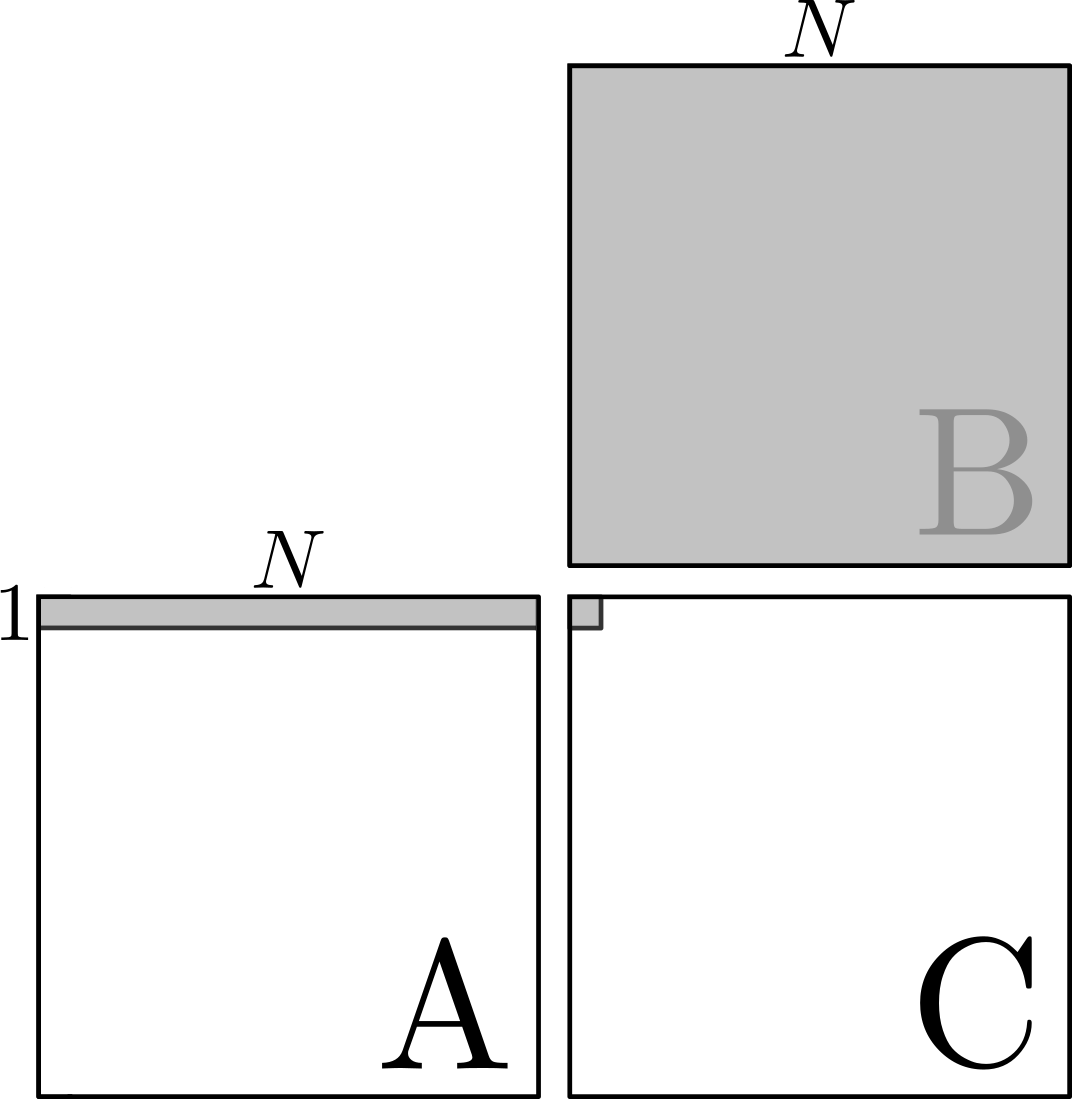
\includegraphics[scale=1]{figures/inner_mmm_n2.png}
  \caption{Local memory size $N^2 + N + 1$}
  \label{fig:innermm_n2}
\end{subfigure}%
\begin{subfigure}{.5\textwidth}
  \centering
  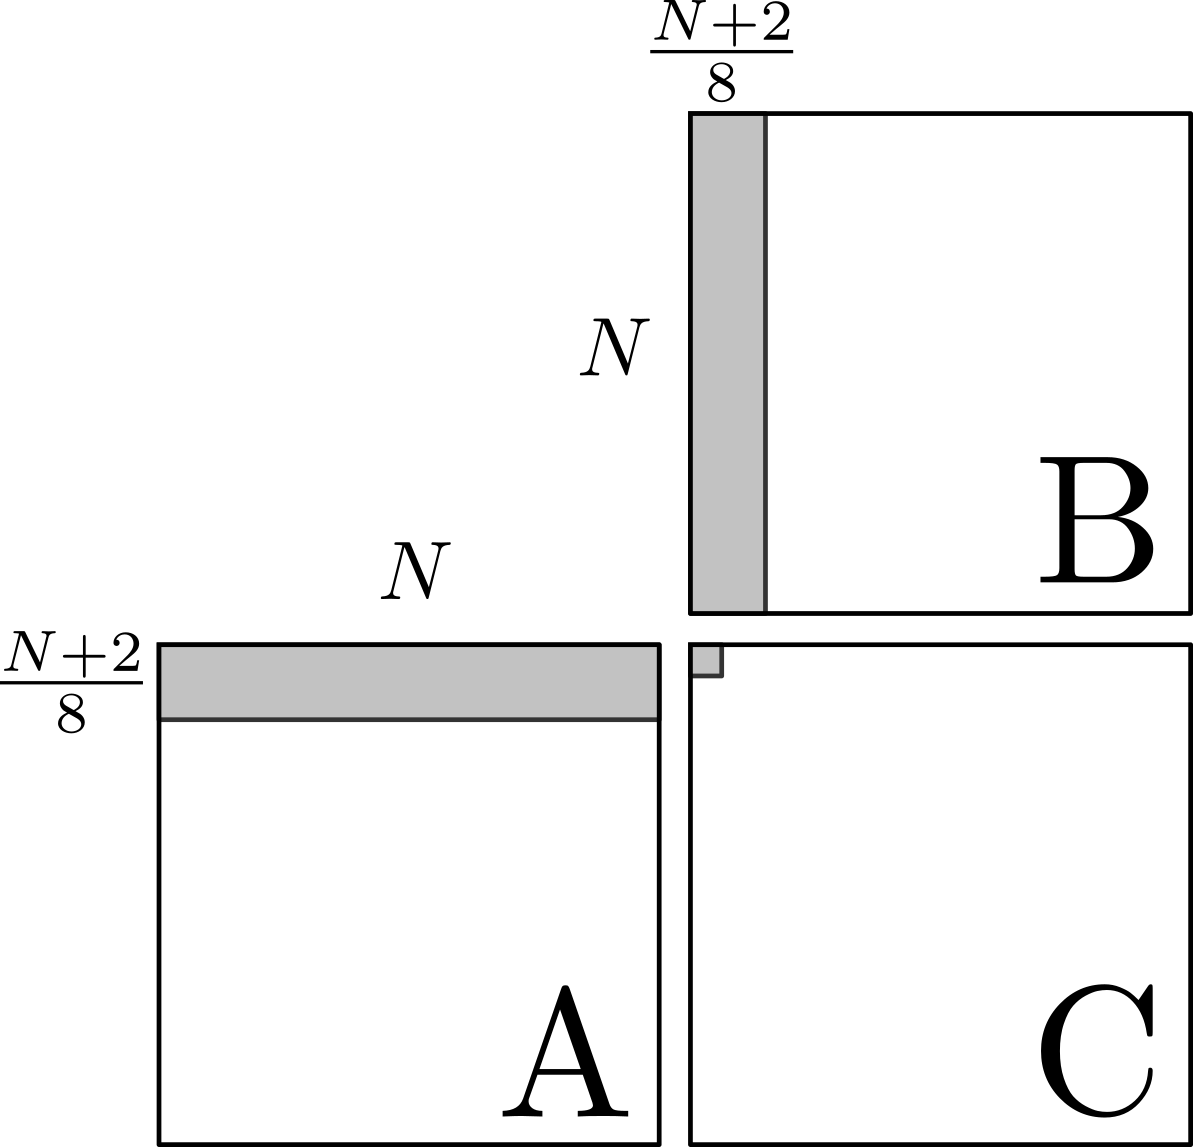
\includegraphics[scale=1]{figures/inner_mmm_n2_4.png}
  \caption{Local memory size  $\frac{N^2}{4} + \frac{N}{2} + 1$}
  \label{fig:innermm_n2_4}
\end{subfigure}
\caption{Inner product MMM from local memory of two sizes.}
\label{fig:innermm}
\end{figure}
\problem{3.1}{5}
Calculate the arithmetic intensity of MMM with inner products when local memory can hold $N^2 + N + 1$ for the scheme where all of $B$, a vector of $A$, and a single element of $C$ (which is being computed) are held in local memory at any time (\Cref{fig:innermm_n2}).
Here we use an inner product scheme: we will entirely compute an individual element of $C$ before moving to the next.

\solution{

$$ \alpha = \frac{(N+(N-1)+1)N^2}{N^2_{B_{read}}+\sum_{m=1}^N(N_{A_{read}[m][1:N]}+\sum_{n=1}^N(1_{C_{read}[m][n]}+1_{C_{write}[m][n]}) ))} = \frac{2N^3}{4N^2} = \frac{N}{2}$$

}

\problem{3.2}{5}
Calculate the arithmetic intensity of MMM with inner products when local memory can hold $\frac{N^2}{4} + \frac{N}{2} + 1$ for the scheme where $\frac{N+2}{8} \times N$ submatrices of $A$, $N \times \frac{N+2}{8}$ submatrices of $B$, and a single element of $C$ (which is being computed) are held in local memory at any time (\Cref{fig:innermm_n2_4}).
We will again be using an inner product scheme: completely compute an individual element of $C$ before moving to the next.


\solution{
\\
\\
Let $\frac{N+2}{8}=p$ (so the blocks are $p\times N$/$N\times p$ and the memory capacity is $2pN+1$.) I'm then going to assume N+2 is a multiple of 8 so that p is a valid integer dimension. (It doesn't actually matter what p is if we just want to understand the general idea of what's going on; all that matters is that we're dealing with some valid block size.) Then say $N=p*q+r$ where q and r are integers and $0\le r<p$. (I.e. q is the max number of whole factors of p that fit into N, and r is the remainder.) This solution is calculated for the naive algorithm where you simply load a block of A and a block of B, then calculate the corresponding block of C, then load the next block of B (keeping A) and compute the next block of C, and keep going until every block of B has been processed. Then move to the next block of A and do the same thing over again (and so on until completed.) In other words, calculate the result of every 
 block of A going into every block of B. The complication in this case is that $q$ of the blocks will be $p\times N$/$N\times p$ but one will be $r\times N$/$N\times r$ (for A and B respectively.)
\begin{align*} 
IO & =  \sum_{l=1}^q\bigg[(pN)_{A_{read}[(l-1)p+1:lp][1:N]} + \sum_{k=1}^q \bigg( (Np)_{B_{read}[1:N][(k-1)p+1:kp]} + \sum_{i=(l-1)p+1}^{lp}\sum_{j=(k-1)p+1}^{kp}(1_{C_{read}[i][j]}+1_{C_{write}[i][j]}) \bigg)   \\
& \;\;\;\;\;\;\;\;\;\;\;\;  + (Nr)_{B_{read}[1:N][qp+1:N]} + \sum_{i=(l-1)p+1}^{lp}\sum_{j=qp+1}^N(1_{C_{read}[i][j]}+1_{C_{write}[i][j]}) \bigg] \\
 & \;\;\;\;\;\;\;\; +
 (rN)_{A_{read}[qp+1:N][1:N]}
  + \sum_{k=1}^q \bigg( (Np)_{B_{read}[1:N][(k-1)p+1:kp]} + \sum_{i=qp+1}^N\sum_{j=(k-1)p+1}^{kp}(1_{C_{read}[i][j]}+1_{C_{write}[i][j]}) \bigg) 
 \\
& \;\;\;\;\;\;\;\; +  (Nr)_{B_{read}[1:N][qp+1:N]} + \sum_{i=qp+1}^N \sum_{j=qp+1}^N (1_{C_{read}[i][j]} + 1_{C_{write}[i][j]}) - N^2*[r==0] \\
& = [qpN+q^2Np+q^22p^2+qNr+q2pr]+ [rN+qNp+q2rp] + [Nr+2r^2]  - N^2*[r==0] \\
& = 2Nqp + 2Nr + 2qpr + 2r^2 + Nq^2p + Nqr + 2q^2p^2 + 2qpr - N^2*[r==0] \\
& = 2N(qp+r) + 2r(qp+r) + Nq(qp+r) + 2qp(qp+r) - N^2*[r==0] \\
& = 2N^2+2Nr+N^2q+2Nqp - N^2*[r==0]\\
& = 2N^2 + 2N(qp+r) + N^2q - N^2*[r==0]\\
& = 4N^2 + N^2\bigg\lfloor\frac{N}{p}\bigg\rfloor - N^2*[r==0]
\end{align*}

Note: Because of the form of this equation, there is a cancellation that will not occur when $r=0$. To get the correct value in this case we must subtract $N^2$. Using this procedure we will recover the correct result that when $p=1$ the number of IO ops is $IO=N^3+3N^2$ and when $p=N$ (and you can store both matrices) $IO=4N^2$. The need to manually subtract $N^2$ when $r=0$ comes simply because there is a loop in my expression that is necessary for the calculation, but becomes invalid (that is it doesn't contribute) when r=0.  

$$ \alpha = \frac{2N^3}{IO} = \frac{2N^3}{4N^2 + N^2\bigg\lfloor\frac{N}{p}\bigg\rfloor - N^2*[r==0]} = \frac{2N}{4+\bigg\lfloor\frac{N}{p}\bigg\rfloor - [r==0]}$$

}

\subsection*{Arithmetic Intensity for Outer Product MMM}

\begin{figure}[H]
\centering
\begin{subfigure}{.5\textwidth}
  \centering
  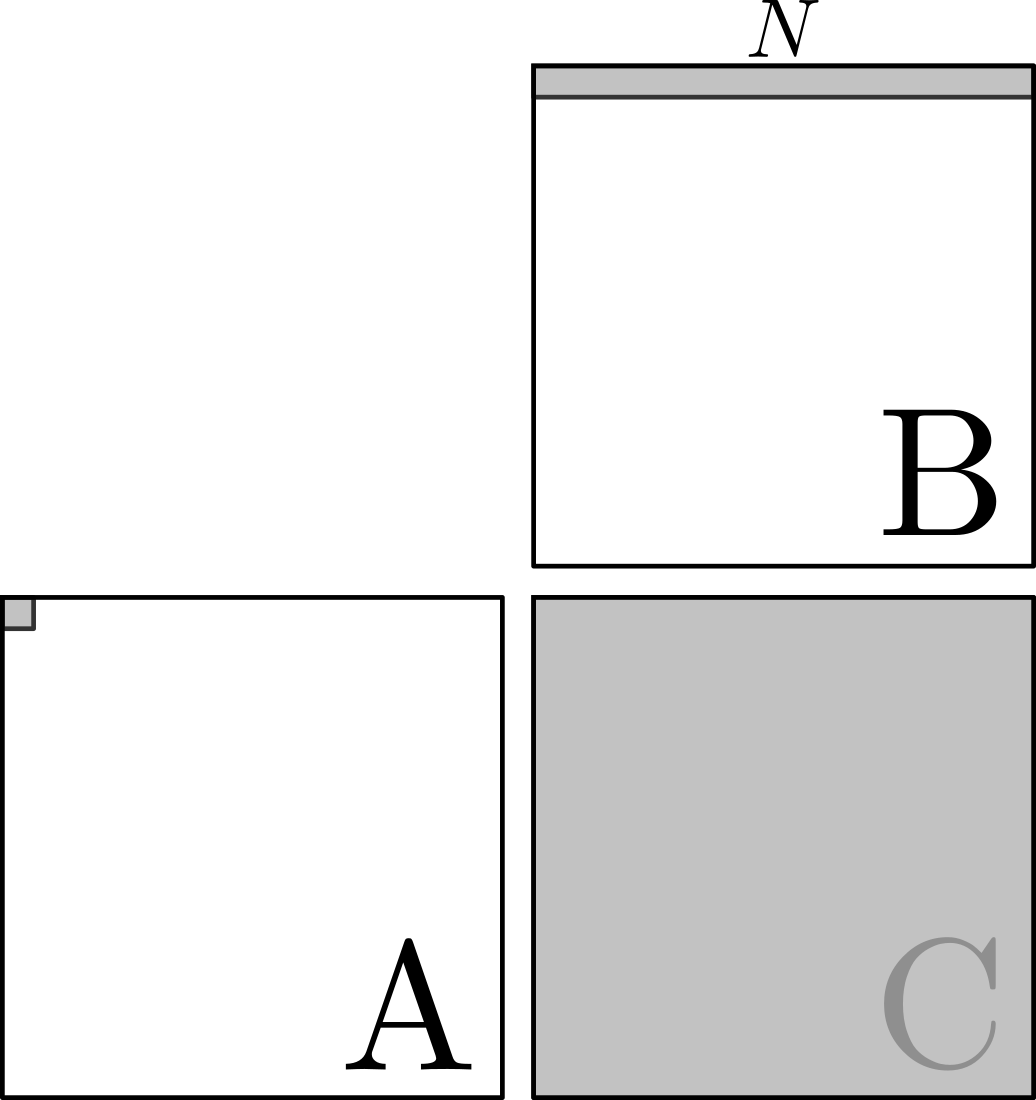
\includegraphics[scale=1]{figures/outer_mmm_n2.png}
  \caption{Local memory size $N^2 + N + 1$}
  \label{fig:outermm_n2}
\end{subfigure}%
\begin{subfigure}{.5\textwidth}
  \centering
  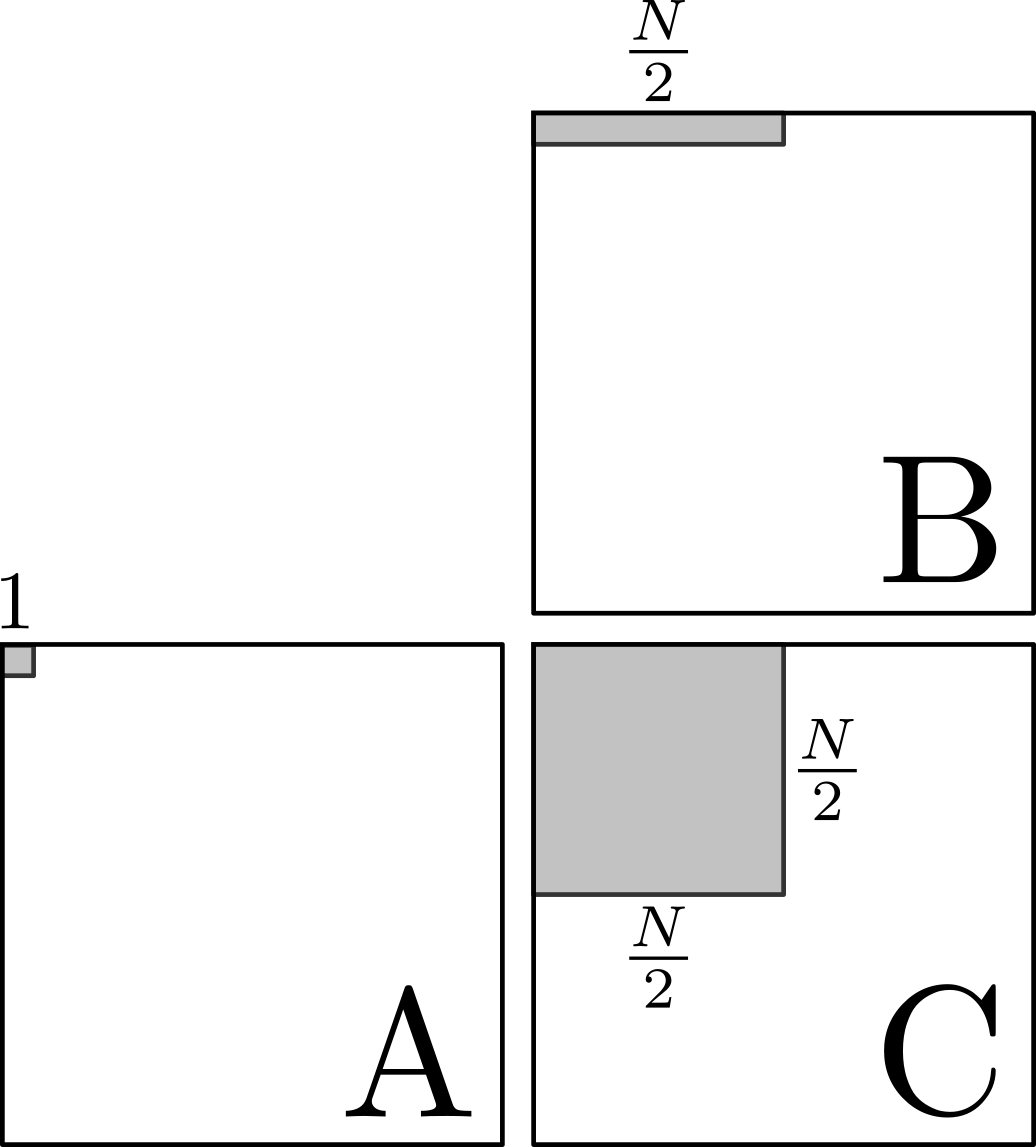
\includegraphics[scale=1]{figures/outer_mmm_n2_4.png}
  \caption{Local memory size  $\frac{N^2}{4} + \frac{N}{2} + 1$}
  \label{fig:outermm_n2_4}
\end{subfigure}
\caption{Outer product MMM from local memory of two sizes}
\label{fig:outermm}
\end{figure}


\problem{3.3}{5}
Calculate the arithmetic intensity of MMM with outer products when local memory can hold $N^2+N +1$ for the scheme where all of $C$, a row of $B$, and a single element of $A$ is held in local memory at any time (\Cref{fig:outermm_n2}).

\solution{

$$\alpha = \frac{(N^2+N^2)N}{N^2_{C_{read}} + \sum_{i=1}^N \big( N_{B_{read}[i][1:N]} +\sum_{j=1}^N 1_{A_{read}[j][i]} \big) + N^2_{C_{write}} } = \frac{2N^3}{4N^2} = \frac{N}{2} $$
}

\problem{3.4}{5}
Calculate the arithmetic intensity of MMM with outer products when local memory can hold $\frac{N^2}{4} + \frac{N}{2} + 1$ for the scheme where we hold a $\frac{N^2}{4}$ block of $C$, a half row of $B$ ($\frac{N}{2}$ elements), and a single element of $A$ in local memory at any time (\Cref{fig:outermm_n2_4}).
Here we use an IO-efficient scheme: we will finish computing an entire $\frac{N}{2} \times \frac{N}{2}$ submatrix of $C$ before writing it back to external memory and starting on the next sub-matrix.

\solution{

For the sake of generality I'm going to compute the result for an arbitrary square block size $l$, and a memory capacity $l^2+l+1$. We can then view the answer to this problem as simply the case where $l=\frac{N}{2}$. Once again to facilitate the calculation I will say: $N=lq+r$, where $l$ and $q$ are integers and $0\le r <l$. (I.e. $q$ and $r$ and are the quotient and remainder of $N/l$.)

\begin{align*} 
IO & = \sum^{q}\bigg( \sum^{q}\bigg(  2l^2_{C_{read/write}} + \sum^{N} \big(l_{B_{read}} + \sum^l 1_{A_{read}}\big)  \bigg) + 2rl_{C_{read/write}} +  \sum^N \big(l_{B_{read}} \sum^r 1_{A_{read}}\big) \bigg)  + \dots \\
   & \;\;\;\;\;\;\;\; + \sum^q \bigg( 2lr_{C_{read}} + \sum^N \big( r_{B_{read}} + \sum^l 1_{A_{read}} \big) \bigg) + 2r^2_{C_{read}} + \sum^N (l_{B_{read}} + \sum^r 1_{A_{read}}) - 2N^2*[r==0] \\
   & = 2q^2l^2 + 2Nq^2l + 2qrl + Nql + Nqr + 2qlr + Nqr + Nql + 2r^2 +2Nr - 2N^2*[r==0] \\
   & = 2Nql + 2Nr + 2qlr + 2r^2 + 2q^2l^2 + 2qlr  + 2Nq^2l + 2Nqr -2N^2*[r==0]\\
   & = 2N(ql+r) + 2r(ql+r) + 2ql(ql+r) + 2Nq(ql+r) -2N^2*[r==0]\\
   & = 2N^2 + 2Nr + 2Nql + 2N^2q -2N^2*[r==0]\\
   & = 2N^2 + 2N(ql+r) + 2N^2q- 2N^2*[r==0]\\
   & = 4N^2 + 2N^2\bigg\lfloor \frac{N}{l} \bigg\rfloor - 2N^2*[r==0]
\end{align*}

$$ \alpha = \frac{2N^3} { IO } = \frac{2N^3}{4N^2 + 2N^2\big\lfloor\frac{N}{l} \big\rfloor - 2N^2*[r==0] } = \frac{N}{2 + \big\lfloor\frac{N}{l} \big\rfloor - [r==0] } $$

Thus we see that when $l=\frac{N}{2}$, $\alpha=\frac{N}{3}$.
}


\subsection*{Comparison of Inner and Outer Products}
\problem{3.5}{5}
Compare your results from Parts 3.1 to 3.3 (inner vs outer product with larger local memory), and your results from Parts 3.2 with 3.4 (inner vs outer product with smaller local memory).
That is, by what factor do the arithmetic intensity of inner and outer product MMMs differ at each memory size?

\solution{ 

For both 3.1 and 3.3 the arithmetic intensity is $\alpha=\frac{N}{2}$. This means that the inner and outer product have the same $\alpha$ (for the algorithms chosen) when the local memory is big enough to hold one of the product matrices, an entire row/vector of the other matrix, and atleast one element of C. This makes sense because in that cause, you don't have to worry about redundantely acessing one of the matrices.
\\

Now comparing 3.2 and 3.4 we see the arithmetic intensities are $\alpha_{inner}=\frac{N}{4+\big\lfloor\frac{N}{p}\big\rfloor- [r==0]}$ and $\alpha_{outer}=\frac{N}{2 + \big\lfloor\frac{N}{l} \big\rfloor - [r==0] }$ respectively. 
We can compare these expressions for a given memory by requiring that $2pN+1=l^2+l+1 \implies 2pN=l(l+1)$. The nicer looking way to satisfy this is to make $p=\frac{l(l+1}{2N}$. A plot of the arithmetic intensities for the block sizes when $p$ and $l$ are related this way is shown below. (N is selected to be $102$ so that $\frac{N+2}{8}=13$ and $\frac{N}{2}=51$ are integers.) 

\begin{figure}[H]
    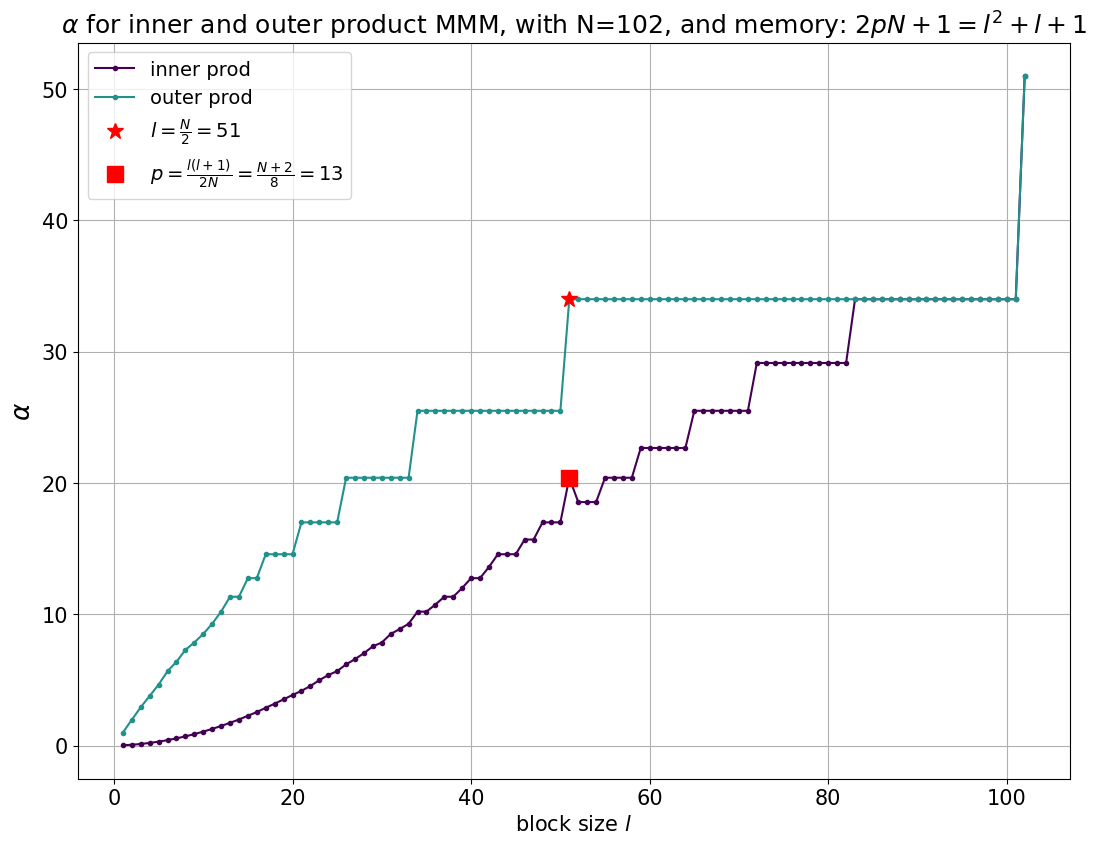
\includegraphics[width=0.85\linewidth]{figures/35_comp.png}
    \centering
    \caption{Comparison of blocking inner and outer product with constant amount of memory. Notice that both intensities approach N/2 as the block size approaches the size of the matrix, which is perfectly consistent with the results of 3.1/3.3. Also note that for the outer product, when the block size is N/2 the intensity is N/3=34 as expected. Similarly, when the block size for the inner product is (N+2)/8  we get the expected result.}
\end{figure}

We can immediately see that for the same amount of memory (when there is not enough memory to store the whole matrix), the outer product does better than the inner product. This is because the outer product has better IO properties.

We also can see steps in intensities which represent the fact that increasing the block size  only helps the arithmetic intensity when it decreases the total number of blocks that have to be loaded, and this only happens when the block-size hits the next-biggest factor of N as it increases. Mathematically this is encoded in the floor functions.
}

\section{MMM Runtimes}
\label{sec:eval}
In this section you will implement MMM with both inner and outer products, execute the code on your VM and report their runtimes.

\subsection*{Implementing Inner Product MMM}
\problem{4.1}{10}
Implement inner product MMM in the function \texttt{inner\_product\_mmm()} contained in \texttt{pa1.cpp}, as described by the following algorithm:
\begin{algorithm}
\SetAlgoLined
\SetInd{0.25em}{0.5em}
\For{$m = 1 \to M$}{
    \For{$n = 1 \to N$}{
        \For{$k = 1 \to K$}{
            $C[m][n] \longleftarrow C[m][n] + A[m][k] \cdot B[k][n]$\;
        }
    }
}
\caption{Inner product MMM}
\label{algo:naivemm-mnk}
\end{algorithm}

\subsection*{Implementing Outer Product MMM}
\problem{4.2}{10}
Implement outer product MMM in the function \texttt{outer\_product\_mmm()} contained in \texttt{pa1.cpp}, as described by the following algorithm:

\begin{algorithm}[H]
\SetAlgoLined
\SetInd{0.25em}{0.5em}
\For{$k = 1 \to K$}{
    \For{$m = 1 \to M$}{
        \For{$n = 1 \to N$}{
            $C[m][n] \longleftarrow C[m][n] + A[m][k] \cdot B[k][n]$\;
        }
    }
}
\caption{Outer product MMM}
\label{algo:naivemm-kmn}
\end{algorithm}

\subsection*{Timing}
\problem{4.3}{15}
With your implementation of the MMM functions, run the provided code.
Plot the run time results, taking the average over 5 iterations.
As mentioned earlier, use only square matrices (i.e., $M = N = K$) to simplify timing comparisons.
The Y-axis should be the run time (in nanoseconds) and X-axis should be the matrix dimension $N$.
Be sure to appropriately label your generated plot with axes, title, and legend.
Your plot must include data for following values of $N$: 16, 32, 64, 128, 256, 512, 1024 (every power of 2 between $2^4$ and $2^{10}$, inclusive).
For plotting, use Python’s \texttt{matplotlib}.
What trends do you see?
Does anything stand out or seem unusual?

\solution{

\begin{figure}[H]
    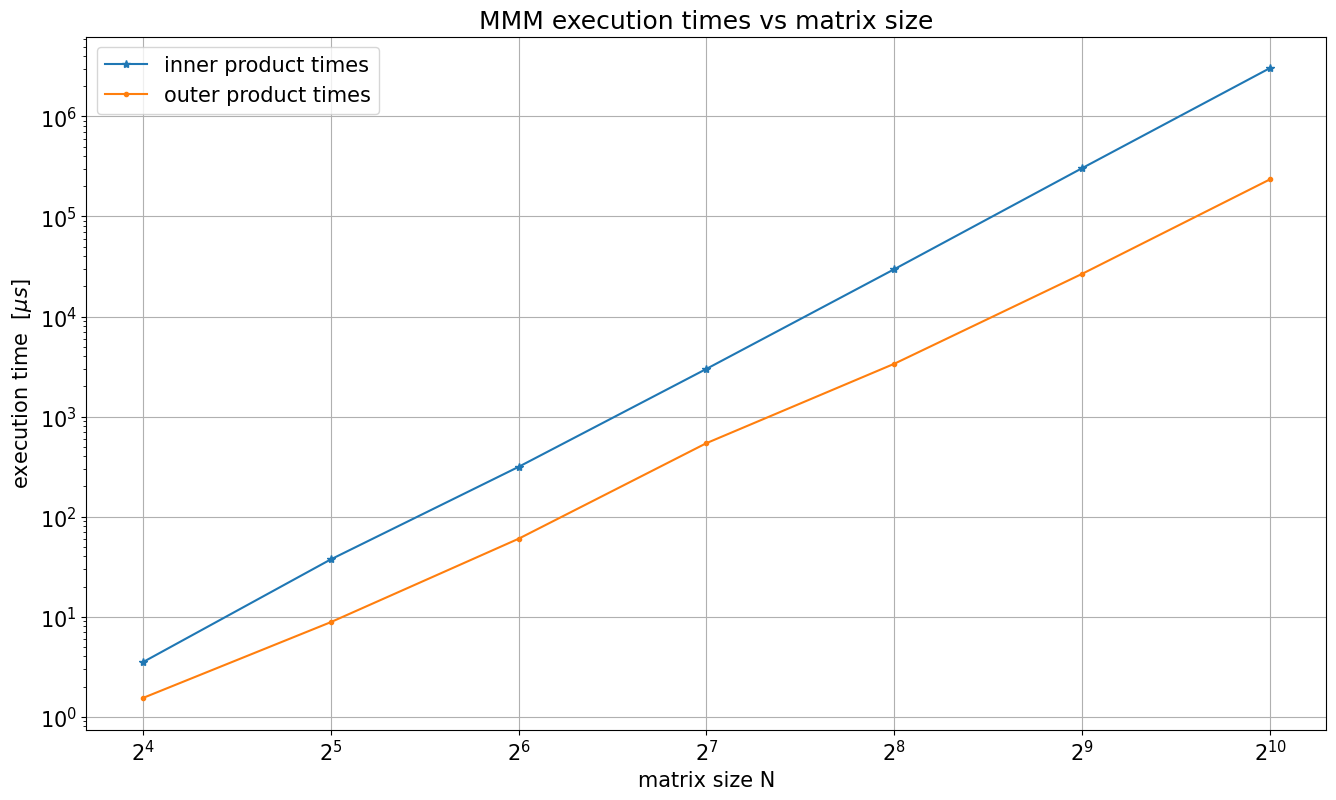
\includegraphics[width=0.85\linewidth]{figures/time_vs_size.png}
    \centering
    \caption{Timings for Part 4}
\end{figure}

We firstly see that the execution time grows in an exponential seeming pattern with respect to matrix size N (given the samples we have, which show a straight line on a log plot.) We also notice that the inner product is has a worse baseline performance than the outer product, but with a similar growth pattern.   

}

\section{Arithmetic Intensity for Convolution}
\label{sec:cnn_ai}
In this section, we will explore the arithmetic intensity of a convolutional layer.
A convolutional layer may be implemented as a matrix-matrix multiplication (MMM) by linearizing the input data tensor and filters into two matrices, respectively. 
For such an implementation, we define the arithmetic intensity of the convolutional layer as the arithmetic intensity of its corresponding MMM.

The size of input data tensor is given as ($I, H, W$), where $I$ is number of input channels, and $H$ and $W$ are the spatial sizes (height and width) of the data tensor. 
The filter tensor of the convolution layers have a size of ($O, I, K, K$), where $O$ is the number of output channels and $K$ is kernel size.
To linearize the data tensor into a data matrix, we first sample several patches from the data tensor with a sampling stride\footnote{The stride is the number of pixels that the filters move on each iteration.} $S$.
Each patch has a size of ($I, K, K$) and is unfolded as a row of the linearized data matrix. 
Note that these patches may overlap one another depending on the kernel size $K \times K$ and stride $S$. 
The size of $S$ is important for determining the size of the linearized data matrix.
Similarly, each filter also has a size of ($I, K, K$) and is unfolded as a column of the linearized filter matrix.
Finally, this convolution layer can be implemented as a matrix-matrix multiplication between the linearized data and filter matrices.
The above process is illustrated in Figure~\ref{fig:conv}.

\begin{figure}
    \centering
    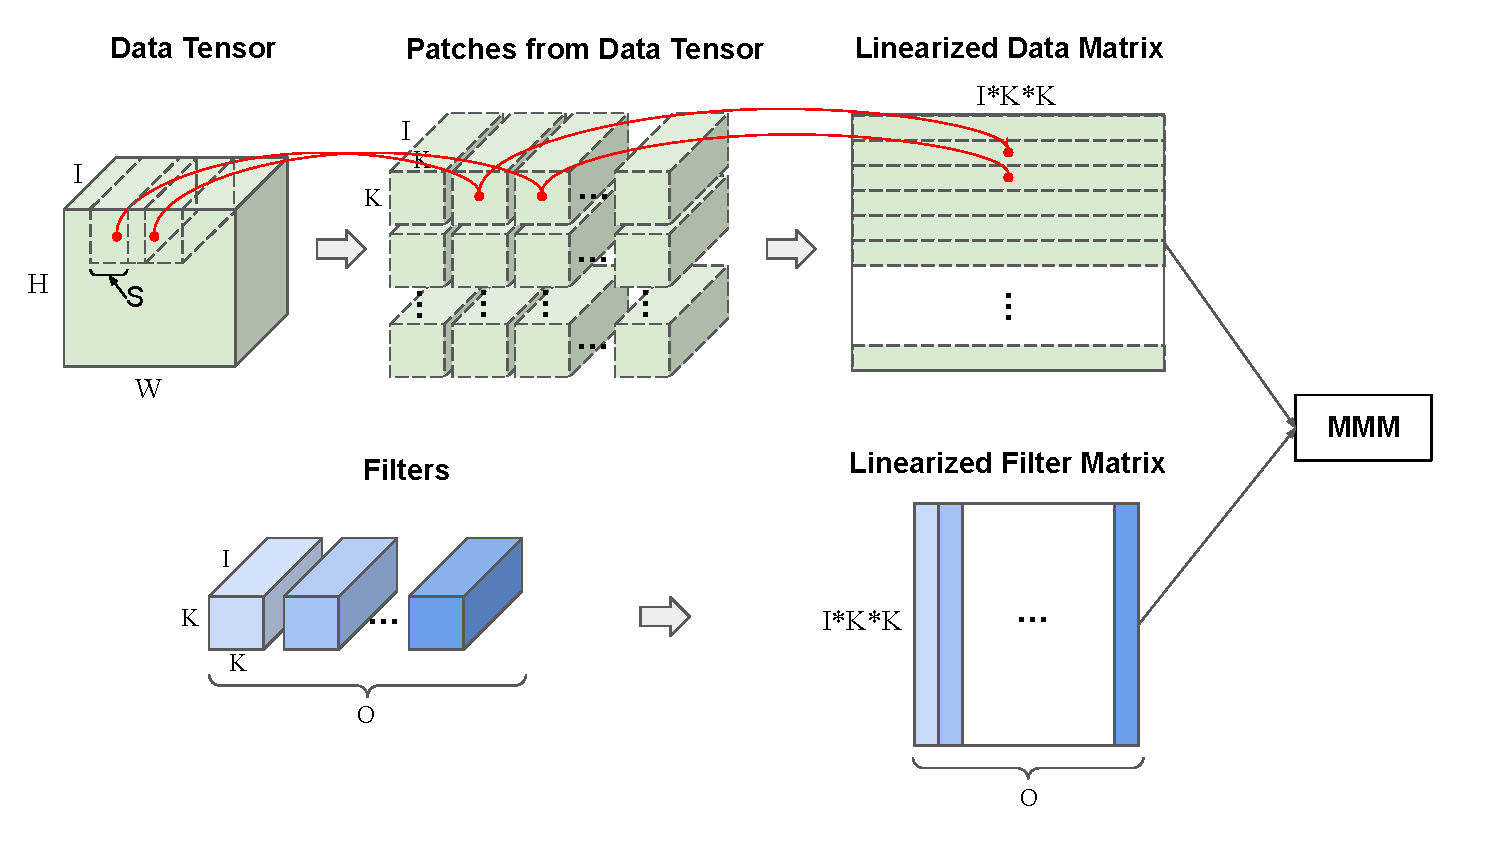
\includegraphics[width=\linewidth]{figures/CS242-Conv.pdf}
    \caption{Overview of a convolution and it's corresponding matrices.}
    \label{fig:conv}
\end{figure}

\problem{5.1}{5}
\begin{enumerate}[label=(\alph*)]
    \item Calculate the IO required for the filter matrix, assuming that the local memory can hold the entire matrix.
    \item Calculate the IO required for the input matrix, assuming that the local memory can hold the entire matrix.
\end{enumerate}

\solution{

For this problem I'm assuming that we're talking about the IO necessary to form the data and filter matrices from their respective tensors. 

\newcommand{\numpatches}{\bigg(\bigg\lceil\frac{W-K}{S}\bigg\rceil+1\bigg)\bigg(\bigg\lceil\frac{H-K}{S}\bigg\rceil+1\bigg)}

\begin{enumerate}
\item[a).] I'm assuming the simplest case, where the entire filter matrix is in local memory and the set of filters are in some external memory. The number of IO operations in this case is simply the number of elements that have to be read, which is: $$IO = IK^2*O$$
\item[b).] In this case I'm assuming the data matrix and a single variable are in local memory and the data tensor is on disk. I'm also assuming the best case where we're smart enough to read a single element of the data tensor into a local variable and then copy it to all the places where we know it will show up in the linearized data matrix. This way we only need to read each element of the data tensor once and the total IO is just the size of the data tensor which is: $$IO=\numpatches*IK^2 $$
To obtain this size for the data tensor, I assumed that the convolution will do an additional shift even if the remaining number of un-convolved elements in a given direction is less than S. This is what gives the ceil functions.  
\end{enumerate}

}

\problem{5.2}{5}
What is the arithmetic intensity for the matrix multiplication between the data matrix and the filter matrix?

\solution{
\newcommand{\numpatches}{\big(\big\lceil\frac{W-K}{S}\big\rceil+1\big)\big(\big\lceil\frac{H-K}{S}\big\rceil+1\big)}

I'm assuming that we can fit the entire result matrix, a row of the filter matrix and an element of the data matrix in memory. We then do the most direct outer-product matrix multiplication. (I'm also including the IO to write the result to disk as part of the calculation.) 

\begin{align} 
\alpha & = \frac{2O \numpatches * IK^2}{ IK^2\big(O +\numpatches\big) + O\numpatches } \\
       & = \frac{2O P IK^2}{IK^2(O+P) + OP}\\
\end{align}
where $P = num patches = \numpatches $
}

\problem{5.3}{5}
How does arithmetic intensity vary with: kernel size ($K$), input channel size ($I$), and stride ($S$)?
Use one or two sentences to describe the trends for each.
Comment on any relationship you notice between $K$ and $S$.
You may find graphs or equations useful in justifying your answer.

\solution{

\begin{figure}[H]
    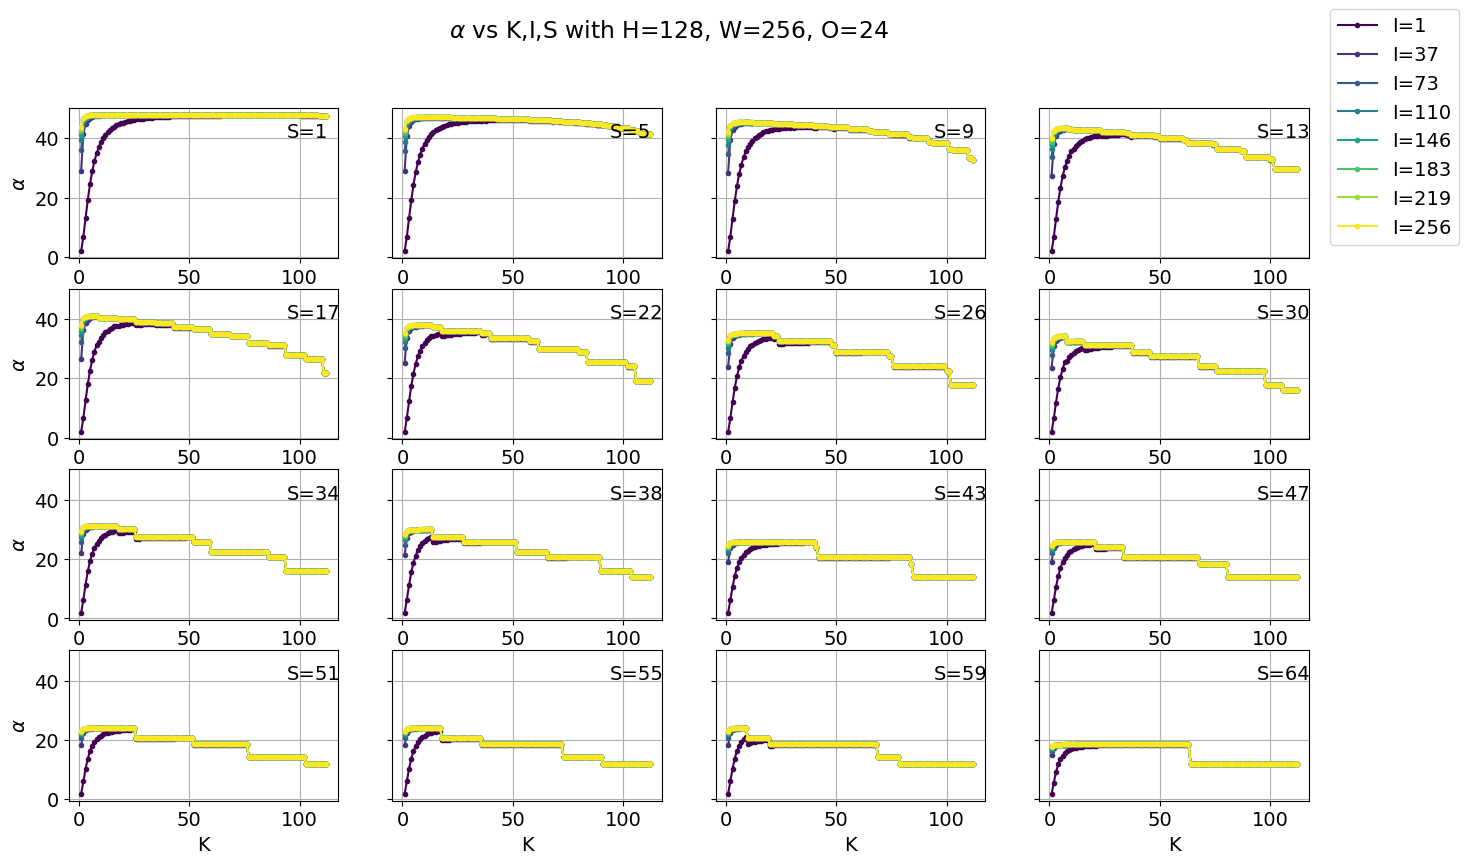
\includegraphics[width=0.95\linewidth]{figures/alpha.png}
    \centering
    \caption{$\alpha$ for Part 5}
\end{figure}

Understanding these results requires remembering that increased $\alpha$ is not the same as decreased absolute computation time. 

At small K, $\alpha$ is large and as K increases $\alpha$ decreases. This makes intuitive sense as a small K corresponds to a smaller filter matrix to load, but a much larger amount of computations because the much bigger size of the data matrix. Also note the discrete downward jumps in $\alpha$ as K increases. These correspond to the fact that increasing K only changes the number of patches when K causes one less factor of S to fit into the matrix at which point the number of convolution patches jumps down and $\alpha$ decreases. 

The channel size I has a large effect on $\alpha$ at small K. Here, larger I corresponds to a larger computational intensity because the increased number of computations outweights the increased amount of IO. We can see this should be true because I multiplies O*P in the numerator but O and P individually in the denominator. However, as K increases the effect of I is diminished.

Lower stride corresponds to greater arithmetic intensity because once again, the effect of lowering the stride is to increase the number computations more quickly than the number of IO operations. 

As stated before, the clear relationship between K and S is that changing the size of K has a bigger impact every time it causes one factor less of S to fit into a dimension of the data matrix. They also both have the same effect on $\alpha$ and increasing S amplifies the importance of changes in K. 
}


\section{What to Submit}
Your submission should be a \texttt{.zip} archive with a \texttt{CS242\_PA\_} prefix followed by each team member's full name separated with two underscores from the next name. The archive should contain:
\begin{itemize}
    \item PDF write-up
    \item Assignment code
\end{itemize}

\noindent
Example filename: \texttt{CS242\_PA1\_Jane\_Doe\_\_John\_Doe\_\_Jane\_Smith\_\_John-Paul\_Smith.zip}\\

\subsection*{Write-up}
Written responses should be contained within a single PDF document.
(\LaTeX~is highly recommended!)
Each response or figure should clearly indicate which problem is being answered.
The write-up must contain the full names of all team members.

\subsection*{Code}
You should include \textbf{all} files that were provided, but with the changes you made.
Additionally, you must include your graphing code and timing data for Part 4.3.


\end{document} 
